\documentclass[10pt,twocolumn]{article}

\usepackage{graphicx}
\usepackage[colorlinks=true,allcolors=blue]{hyperref}

\begin{document}

\title{Next-generation design tools for intelligent transportation systems}
\author{Dominik Ascher and Georg Hackenberg}
\maketitle

\begin{abstract}
    TODO
\end{abstract}

\section{Introduction}
\label{sec:introduction}

The transformative patterns of future mobility are fundamentally enabled through interconnected and integrated systems.
As such, Intelligent Transportation Systems (ITS) integrate new transportation paradigms such as connected and autonomous vehicles (CAV), multi-modal and demand-responsive transport systems, as well as electric vehicles and the transportation electrification. For this, complex scenarios and requirements need to be holistically addressed, from which integrated system designs have to be derived, which allow transport infrastructures and their heterogenous actors to be more efficient and sustainable.

Therefore, constituent systems need to be designed with respect to most efficient structures and control strategies within themselves, while accounting for and exploiting the emergent properties they achieve in conjunction and interdependence with other systems, as a composed, integrated system-of-systems (SoS). To systematically support the aforementioned systems engineering task, model- and simulation-based systems engineering~\cite{gianni2014modeling} can be employed for abstraction of design problems through the use of system models and their evaluation, i.e. their numerical approximation in terms of concrete behavior at run time. For this, well-defined system models are formulated, for which then simulation aids projecting and obtaining information and performance metrics about the system under design and its environment. Therefore, both structural as well as behavioral system design tasks can be supported using a overarching system design methodology at design time as well as run time.

In terms of benefits, on the one hand side, system models faciliate gaining improved system understanding through specification, while allowing rapid system modification through defined variation points for designing a system. On the other hand side, simulation aids approximating information about the system dynamics and performance of a system under design.

For this, in previous work, we established an integrated systems modeling technique for integrated transportation and power systems. Here, our systems modeling technique allows one to model both transportation and power system scenarios, as well as mobility-on-demand scenarios to assess system design options systemtically and improve system understanding holistically, based on a formal foundation~\cite{ascher_hackenberg_2014,ascher_hackenberg_2015,ascher_hackenberg_2016,ascher_hackenberg_2017}




\subsection{Research objective}

With our research, we want to help improve the efficiency and effectiveness of today's transportation systems.
To achieve this goal, we work on methodologies for designing such systems and verifying their properties.
Fundamentally, we promote a formal approach capturing the relevant design decisions and their relations.
Furthermore, we integrate scenario-based simulation of system dynamics and evaluation of emergent properties.
Finally, we exploit optimization algorithms for optimizing system dynamics as well as static design decisions.

\subsection{Research question}

In this paper, we ask how the next generation of design tools for intelligent transportation systems should look like.
Therefore, first we want to understand which system properties and design decisions should be represented in these tools.
Then, we want to learn how the design decisions could be verified with respect to the desired system properties.
Finally, we want to study how the relevant design information could be represented in a graphical user interface.

\subsection{Research methodology}

In the following, we first propose a modeling and simulation framework for capturing design decisions and evaluating emergent properties in Section~\ref{sec:framework}.
Then, we propose a graphical user interface for building system designs, starting simulation runs, and visualizing simulation outcomes in Section~\ref{sec:gui}.
Thereafter, we propose two special applications of our modeling and simulation framework as well as user interface technology in Section~\ref{sec:application}.
Finally, we draw our conclusions and describe future direction of research and development on the design of ITS in Section~\ref{sec:conclusion}. 

\section{Underlying framework}
\label{sec:framework}

In this section, we propose a modeling and simulation framework for the design of intelligent transportation systems.
We first introduce a modeling technique for describing the design decisions and defining evaluation scenarios in Section~\ref{sec:modeling-technique}.
Then, we propose an interface for implementing and integrating custom control strategies in Section~\ref{sec:controller-interface}.
Finally, we define an interface for collecting statistics during simulation of system dynamics in Section~\ref{sec:statistics-interface}.

\subsection{Modeling technique}
\label{sec:modeling-technique}
The scope of our underlying modeling technique is based on integrated transportation system modeling techniques, which allow assessment of integrated, electrified ITS systems for the purpose of designing emergent  integrated system properties. The approach allows one to model integrated transportation system problems on a mesoscopic to microscopic level, \cite{ascher_hackenberg_2014, ascher_hackenberg_2015}, supported by a formal systems modeling foundation \cite{ascher_hackenberg_2016, ascher_hackenberg_2017}. In terms of considered domain problems, for instance, future transportation electrification as well as demand-responsive transport scenarios may be investigated.

\subsubsection{Scope}
For this, our modeling technique supports different design tasks. Here, our modeling technique supports deriving well-defined designs of transportation systems as well as designing control strategies in the context of on-demand transportation problems.

Static Property Optimization concerns optimization of infrastructure properties.
Dynamic Property Optimization concerns optimization of control strategies.
Mixed Property Optimization concerns both optimization of infrastructures and control strategies. 

\subsubsection{Formalism}
Currently, our modeling technique is based on a formalism for Discrete-Event Simulation (DES) ~\cite{fishman2001discrete}, where Figure~\ref{fig:modeling-technique} provides an overview of main domain concepts, where t formalism is intended to capture a concise and an essential set of static properties, static calculations, and dynamic states as well as events for establishing sound models and control strategies for on-demand transportation systems.

Each concept is described in terms of their static (i.e.\ time-independent) properties and calculations as well as their dynamic (i.e.\ time-dependent) state functions typically sampled during computer simulations. In addition, we define events as functions over a system's trajectory of states, which precisely indicate when actions need to be taken in the system simulation. Thus, events significantly reduce simulation complexity by limiting action space dimensionality and by abstracting from discrete-time resolutions. 

In terms of considered domain concepts for the formalism, we use intersections $i \in I$, segments $s \in S$ as well as locations $l \in L$ for describing properties about the transportation infrastructure.
Based on the transportation infrastructure, we use charging stations $cs \in CS$ for describing the charging infrastructure. In addition, we describe transportation demands $d \in D$ on the transportation infrastructure. 
Finally, we use vehicles $v \in V$ for describing transportation supply and capacities.


\begin{figure*}[tbp]
    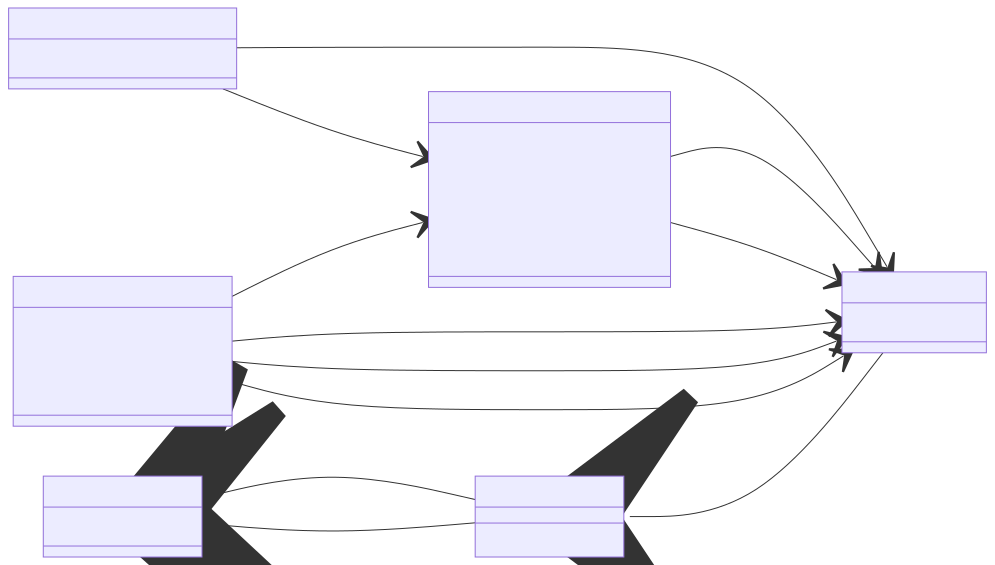
\includegraphics[width=\textwidth]{../../diagrams/model/classes-v0.1.png}
    \caption{Modeling technique}
    \label{fig:modeling-technique}
\end{figure*}

TODO

\subsection{Controller interface}
\label{sec:controller-interface}

TODO

\begin{figure*}[tbp]
    \includegraphics[width=\textwidth]{../../diagrams/controller/classes.png}
    \caption{Controller interface}
    \label{fig:controller-interface}
\end{figure*}

TODO

\subsubsection{Manual controller}

TODO

\subsubsection{Random controller}

TODO

\subsubsection{Greedy controller}

TODO

\subsubsection{Smart controller}

TODO

\subsubsection{Switchable controller}

TODO

\subsection{Statistics interface}
\label{sec:statistics-interface}

TODO

\begin{figure}[htbp]
    \includegraphics[width=\columnwidth]{../../diagrams/statistics/classes.png}
    \caption{Statistics interface}
    \label{fig:statistics-interface}
\end{figure}

TODO

\section{Graphical user interface}
\label{sec:gui}

TODO

\begin{figure*}[tbp]
    \includegraphics[width=\textwidth]{../../screenshots/basic-simulation.png}
    \caption{Graphical user interface}
    \label{fig:gui}
\end{figure*}

TODO

\subsection{Map}

TODO

\subsection{Vehicle charts}

TODO

\subsubsection{Vehicle battery chart}

TODO

\subsubsection{Vehicle distance chart}

TODO

\subsection{Demand charts}

TODO

\subsubsection{Demand time chart}

TODO

\subsubsection{Demand distance chart}

TODO

\subsection{Infrastructure charts}

TODO

\subsubsection{Intersection chart}

TODO

\subsubsection{Segment chart}

TODO

\subsubsection{Station chart}

TODO

\section{Specific applications}
\label{sec:application}

TODO

\subsection{Controller comparison}
\label{sec:controller-comparison}

TODO

\begin{figure*}[tbp]
    \includegraphics[width=\textwidth]{../../screenshots/controller-comparison.png}
    \caption{Controller comparison}
    \label{fig:controller-comparison}
\end{figure*}

TODO

\subsection{Infrastructure comparison}
\label{sec:infrastructure-comparison}

TODO

\begin{figure*}[tbp]
    \includegraphics[width=\textwidth]{../../screenshots/infrastructure-comparison.png}
    \caption{Infrastructure comparison}
    \label{fig:infratructure-comparison}
\end{figure*}

TODO

\section{Conclusion}
\label{sec:conclusion}

TODO

\bibliographystyle{plain}
\bibliography{main}

\end{document}